\documentclass[dvipsnames]{beamer}  

\mode<presentation>
{
  \usetheme{Singapore}
  % or ...
  \setbeamercovered{transparent}
  % or whatever (possibly just delete it)
}

\setbeamercolor{block body}{fg=black, bg=green!10}

\usepackage{fontspec} 
\usepackage[mathscr]{euscript} 
%\usepackage[xcharter]{newtxmath}
%\setmainfont{XCharter}
\setmonofont{DejaVu Sans Mono}[Scale=MatchLowercase] % provides unicode characters 


\usefonttheme{professionalfonts}
%\usepackage[english]{babel}
% or whatever
%\usepackage[latin1]{inputenc}
% or whatever
%\usepackage{times}
\usepackage[T1]{fontenc}
% Or whatever. Note that the encoding and the font should match. If T1
% does not look nice, try deleting the line with the fontenc.

%%%%%%%%%%%%%%%%%%%%%% start my preamble %%%%%%%%%%%%%%%%%%%%%%
\renewcommand{\insertnavigation}[1]{}

\addtobeamertemplate{navigation symbols}{}{%
    \usebeamerfont{footline}%
    \usebeamercolor[fg]{footline}%
    \hspace{1em}%
    \insertframenumber/\inserttotalframenumber
    \vspace{0.5em}
}

\setbeamercolor{footline}{fg=blue}
\setbeamerfont{footline}{series=\bfseries}

%\setbeamertemplate{mini frames}{}

%\usepackage{adjustbox}
\usepackage{graphicx}
\usepackage{amsmath, amssymb, amsthm}
\usepackage{mathtools}

\usepackage{fancyvrb}

\usepackage{hyperref}

\usepackage{mathrsfs} % fonts, caligraphic
\usepackage{bbm}

% tikz
\usepackage{tikz}
\usepackage{tikz-cd}
\usetikzlibrary{positioning}
\usetikzlibrary{arrows}
\usetikzlibrary{calc}
\usetikzlibrary{intersections}
\usetikzlibrary{matrix}
\usetikzlibrary{decorations}
\usetikzlibrary{shapes, fit}
\usetikzlibrary{arrows.meta}
\usetikzlibrary{decorations.pathreplacing}  %for brac

\usepackage{pgf}
\usepackage{pgfplots}
\pgfplotsset{compat=1.7}


\usepackage{graphviz}

%\usepackage[usenames, dvipsnames]{color}


% nice inequalities
\renewcommand{\leq}{\leqslant}
\renewcommand{\geq}{\geqslant}


\setlength{\parskip}{1.5ex plus0.5ex minus0.5ex}
\setlength{\jot}{12pt} 

\usepackage[ruled, lined]{algorithm2e}


\definecolor{pale}{RGB}{235, 235, 235}
\definecolor{pale2}{RGB}{175,238,238}
\definecolor{turquois4}{RGB}{0,134,139}
\definecolor{DarkOrange1}{RGB}{255,127,0}

\newcommand{\emp}[1]{\textcolor{DarkOrange1}{\bf #1}}
\newcommand{\newtopic}[1]{\textcolor{Green}{\Large \bf #1}}
\newcommand{\navy}[1]{\textcolor{Blue}{\bf #1}}
\newcommand{\navymth}[1]{\textcolor{Blue}{#1}}
\newcommand{\red}[1]{\textcolor{red}{#1}}

% Minted
\definecolor{bg}{rgb}{0.95,0.95,0.95}
\usepackage{minted}
\usemintedstyle{friendly}
\newminted{python}{mathescape,frame=lines,framesep=4mm,bgcolor=bg}
\newminted{ipython}{mathescape,frame=lines,framesep=4mm,bgcolor=bg}
\newminted{julia}{mathescape,frame=lines,framesep=4mm,bgcolor=bg}
\newminted{c}{mathescape,frame=lines,framesep=4mm,bgcolor=bg}
\renewcommand{\theFancyVerbLine}{\sffamily
    \textcolor[rgb]{0.5,0.5,1.0}{\scriptsize {\arabic{FancyVerbLine}}}}


\definecolor{Brown}{rgb}{0.59, 0.29, 0.0}
\newcommand{\Fact}{\textcolor{Brown}{\bf Fact. }}
\newcommand{\Thm}{\textcolor{Brown}{\bf Theorem. }}
\newcommand{\Eg}{\textcolor{ForestGreen}{Example. }}
\newcommand{\Egs}{\textcolor{ForestGreen}{Examples. }}
\newcommand{\Ex}{{\bf Ex. }}

\newcommand{\CC}{\mathbbm C}
\newcommand{\EE}{\mathbbm E}
\newcommand{\FF}{\mathbbm F}
\newcommand{\RR}{\mathbbm R}
\newcommand{\KK}{\mathbbm K}
\newcommand{\MM}{\mathbbm M}
\newcommand{\NN}{\mathbbm N}
\newcommand{\PP}{\mathbbm P}
\newcommand{\TT}{\mathbbm T}
\newcommand{\QQ}{\mathbbm Q}
\newcommand{\WW}{\mathbbm W}
\newcommand{\VV}{\mathbbm V}
\newcommand{\ZZ}{\mathbbm Z}

\newcommand{\Asf}{\mathsf A}
\newcommand{\Esf}{\mathsf E}
\newcommand{\Fsf}{\mathsf F}
\newcommand{\Gsf}{\mathsf G}
\newcommand{\Msf}{\mathsf M}
\newcommand{\Lsf}{\mathsf L}
\newcommand{\Nsf}{\mathsf N}
\newcommand{\Psf}{\mathsf P}
\newcommand{\Qsf}{\mathsf Q}
\newcommand{\Ssf}{\mathsf S}
\newcommand{\Tsf}{\mathsf T}
\newcommand{\Xsf}{\mathsf X}
\newcommand{\Ysf}{\mathsf Y}
\newcommand{\Vsf}{\mathsf V}
\newcommand{\Wsf}{\mathsf W}
\newcommand{\Zsf}{\mathsf Z}

\newcommand{\aA}{\mathscr A}
\newcommand{\bB}{\mathscr B}
\newcommand{\cC}{\mathscr C}
\newcommand{\dD}{\mathscr D}
\newcommand{\eE}{\mathscr E}
\newcommand{\gG}{\mathscr G}
\newcommand{\hH}{\mathscr H}
\newcommand{\iI}{\mathscr I}
\newcommand{\fF}{\mathscr F}
\newcommand{\lL}{\mathscr L}
\newcommand{\pP}{\mathscr P}
\newcommand{\rR}{\mathscr R}
\newcommand{\sS}{\mathscr S}
\newcommand{\vV}{\mathscr V}
\newcommand{\wW}{\mathscr W}
\newcommand{\mM}{\mathscr M}
\newcommand{\oO}{\mathscr O}
\newcommand{\zZ}{\mathscr Z}

\newcommand{\bP}{\mathbf P} 
\newcommand{\bR}{\mathbf R}
\newcommand{\bQ}{\mathbf Q}


%%%%%% special symbols %%%%%%%%%%

\newcommand{\volone}{Volume~I}
\newcommand{\voltwo}{Volume~II}

% transpose, not currently using
\newcommand\T{{\mathpalette\raiseT\intercal}}
\newcommand\raiseT[2]{\raisebox{0.25ex}{$#1#2$}}

% nice inequalities
\renewcommand{\leq}{\leqslant}
\renewcommand{\geq}{\geqslant}

% nice greek letters
\renewcommand{\phi}{\varphi}
\renewcommand{\epsilon}{\varepsilon}

% inner product
\providecommand{\inner}[1]{\left\langle{#1}\right\rangle}

% set of matrices
\newcommand{\matset}[2]{ \MM^{ #1 \times #2 } }

% stochastic dominance
\newcommand{\lefsd}{\preceq_{\textrm{F}}}
\newcommand{\lessd}{\preceq_{\textrm{S}}}

% argmax and min
\newcommand{\argmax}{\operatornamewithlimits{argmax}}
\newcommand{\argmin}{\operatornamewithlimits{argmin}}

% sets and logic
\newcommand{\st}{\ensuremath{\ \mathrm{s.t.}\ }}
\newcommand{\setntn}[2]{ \{ #1 : #2 \} }
\newcommand{\natset}[1]{[ #1 ]}

% some useful symbols
\newcommand{\given}{\, | \,}
\newcommand{\cf}[1]{ \lstinline|#1| }
\newcommand{\fore}{\therefore \quad}
\newcommand{\1}{\mathbbm 1}
\newcommand{\me}{\mathrm{e}}               % Euler's e
\newcommand*\diff{\mathop{}\!\mathrm{d}}   % d for integrals

% shortcuts
\newcommand{\la}{\langle}
\newcommand{\ra}{\rangle}

% relations
\newcommand{\eqdist}{\stackrel{d} {=} }
\newcommand{\iidsim}{\stackrel{\textrm{ {\sc iid }}} {\sim} }

% convergence
\newcommand{\tod}{\stackrel { d } {\to} }
\newcommand{\tow}{\stackrel { w } {\to} }
\newcommand{\toprob}{\stackrel { p } {\to} }
\newcommand{\toms}{\stackrel { ms } {\to} }


%%%%%%%%%%% operators %%%%%%%%%%%%

\DeclareMathOperator{\fix}{fix}  % exponential draw
\DeclareMathOperator{\Exp}{Exp}  % exponential draw
\DeclareMathOperator{\Lip}{Lip}
\DeclareMathOperator{\cl}{cl}
\DeclareMathOperator{\graph}{graph}
\DeclareMathOperator{\interior}{int}
\DeclareMathOperator{\Prob}{Prob}
\DeclareMathOperator{\determinant}{det}
\DeclareMathOperator{\trace}{trace}
\DeclareMathOperator{\sgn}{sgn}
\DeclareMathOperator{\Span}{span}
\DeclareMathOperator{\diag}{diag}
\DeclareMathOperator{\proj}{proj}
\DeclareMathOperator{\rank}{rank}
\DeclareMathOperator{\kernel}{null}
\DeclareMathOperator{\cov}{Cov}
\DeclareMathOperator{\corr}{Corr}
\DeclareMathOperator{\var}{Var}
\DeclareMathOperator{\mse}{mse}
\DeclareMathOperator{\se}{se}
\DeclareMathOperator{\range}{range}
\DeclareMathOperator{\dimension}{dim}
\DeclareMathOperator{\epi}{epi}
\DeclareMathOperator{\vecop}{vec}

\DeclareMathOperator{\real}{Re}
\DeclareMathOperator{\imag}{Im}

\DeclareMathOperator{\csum}{cs} % column sum
\DeclareMathOperator{\rsum}{rs} % row sum



\hypersetup{
    linkcolor=Blue,
    colorlinks=true,
    filecolor=magenta,      % color of file links
    urlcolor=cyan           % color of external links
}


\subtitle{A Quick Course in Dynamic P}

\begin{document}

\begin{frame}
  \titlepage
\end{frame}


\begin{frame}
    
    Loosely based on


    \begin{itemize}
        \item \href{https://dp.quantecon.org}{Dynamic Programming: Foundations}
            by Thomas Sargent and John Stachurski
            \vspace{0.5em}
        \item \href{https://arxiv.org/abs/2308.02148}{Completely Abstract Dynamic Programming}
            by Thomas Sargent and John Stachurski
    \end{itemize}


            \vspace{0.5em}
            \vspace{0.5em}
            \vspace{0.5em}
            \vspace{0.5em}
            \vspace{0.5em}
    Inspired by
    %
    \begin{itemize}
        \item \href{https://web.mit.edu/dimitrib/www/Abstract_DP_2ND_EDITION_Complete.pdf}{Abstract Dynamic Programming} by Dimitri Bertsekas
    \end{itemize}


\end{frame}


\begin{frame}
    \frametitle{Topics}

    Handling a large range of dynamic programs

    \begin{itemize}
        \item state-dependent discounting
            \vspace{0.5em}
        \item recursive preferences
            \vspace{0.5em}
        \item quantile preferences
            \vspace{0.5em}
        \item adversarial agents, ambiguity, continuous time, etc., etc.
    \end{itemize}


            \vspace{0.5em}
            \vspace{0.5em}
    Generalization $\implies$ abstraction $\implies$ clearer proofs 

    \begin{itemize}
        \item clarifies optimality conditions
            \vspace{0.5em}
        \item clarifies relationships between DPs
    \end{itemize}

\end{frame}


\begin{frame}
    \frametitle{Omitted}

    Approximation methods

    \begin{itemize}
        \item interpolation
            \vspace{0.5em}
        \item orthogonal projection
            \vspace{0.5em}
        \item kernel averages
            \vspace{0.5em}
        \item neural nets
    \end{itemize}



    How do they interact with the algorithms described below?

    Some answers in
    %
    \begin{itemize}
        \item Neurodynamic programming (Bertsekas \& Tsitsiklis, 1996)
            \vspace{0.5em}
        \item Subsequent literature
            \vspace{0.5em}
        \item DP book Vol 2...?
    \end{itemize}
    

\end{frame}


\begin{frame}
    \frametitle{Prelude: a standard model}

    Consider a \navy{Markov decision process} (MDP) with
    %
    \begin{enumerate}
        \item a finite set $\Xsf$ called the \navy{state space} and
        \vspace{0.5em}
        \item a finite set $\Asf$ called the \navy{action space}
    \end{enumerate}
     
    \vspace{0.5em}
        \vspace{0.5em}
        \vspace{0.5em}

    Actions are restricted by a \navy{feasible correspondence} $\Gamma$

    \begin{itemize}
        \vspace{0.5em}
        \item from $\Xsf$ to $\Asf$
        \vspace{0.5em}
        \item $\Gamma(x) =$ actions available in state $x$  (nonempty)
    \end{itemize}

\end{frame}


\begin{frame}

    \begin{itemize}
        \item next period state $x'$ is drawn from $P(x,a, \cdot)$
    \vspace{0.5em}
        \item flow \navy{reward} at $(x, a)$ is $r(x, a)$ 
    \vspace{0.5em}
        \item constant \navy{discount factor} $\beta \in (0,1)$
    \end{itemize}


        \vspace{0.5em}
        \vspace{0.5em}

    \navy{Lifetime rewards} are
    %
    \begin{equation*}
        \EE \sum_{t \geq 0}
        \beta^t r(X_t, A_t)
    \end{equation*}
    %

    \vspace{0.5em}
    \vspace{0.5em}
    The \navy{Bellman equation} is
    %
    \begin{equation*}
            v(x)
            = \max_{a \in \Gamma(x)}
            \left\{
                r(x, a)
                + \beta
                \sum_{x'} v(x') P(x, a, x')
            \right\}
    \end{equation*}

\end{frame}



\begin{frame}
    

    A \navy{feasible policy} is a map $\sigma \colon \Xsf \to \Asf$ with
    %
    \begin{equation*}
        \sigma(x) \in \Gamma(x)
        \quad \text{for all} \quad
        x \in \Xsf
    \end{equation*}

    \begin{itemize}
        \item $\Sigma := $ all feasible policies
    \end{itemize}


    \vspace{0.5em}
    \vspace{0.5em}
    \vspace{0.5em}
    \vspace{0.5em}

    Feasible policy $\sigma$ is called \navy{$v$-greedy} if
    %
    \begin{equation*}
        \sigma(x) \in             
        \argmax_{a \in \Gamma(x)}
        \left\{
            r(x, a)
            + \beta
            \sum_{x'} v(x') P(x, a, x')
        \right\}
        \quad \forall \, x \in \Xsf
    \end{equation*}

\end{frame}




\begin{frame}
    

    \vspace{0.5em}
    The \navy{Bellman operator} is
    %
    \begin{equation*}
        (Tv)(x)
            = \max_{a \in \Gamma(x)}
            \left\{
                r(x, a)
                + \beta
                \sum_{x'} v(x') P(x, a, x')
            \right\}
    \end{equation*}

    \vspace{0.5em}
    \vspace{0.5em}
    For each $\sigma \in \Sigma$, we introduce the \navy{policy operator} 
    %
    \begin{equation*}
        (T_\sigma \, v)(x) 
            = r(x, \sigma(x))
            + \beta
            \sum_{x'} v(x') P(x, \sigma(x), x')
    \end{equation*}


    \vspace{0.5em}
    \vspace{0.5em}

    Note:
    %
    \begin{equation*}
        \sigma \text{ is $v$-greedy}
        \quad \iff \quad
        Tv = T_\sigma \, v
    \end{equation*}

\end{frame}


\begin{frame}

    \begin{figure}
        \centering
        \scalebox{0.5}{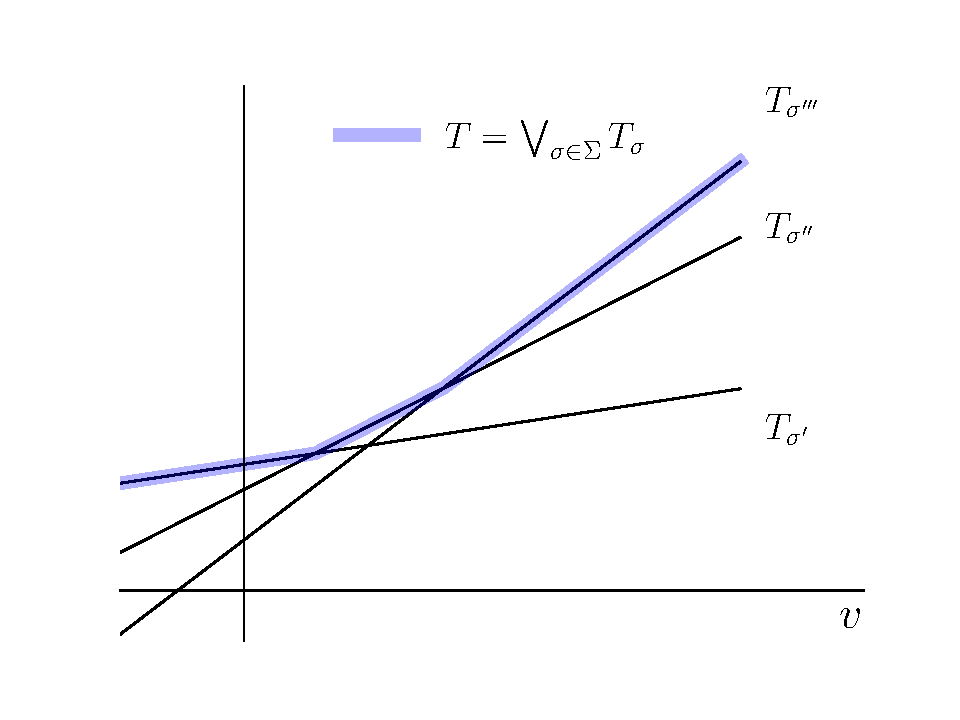
\includegraphics{bellman_envelope.pdf}}
        \caption{\label{f:bellman_envelope} $T$ is the pointwise max.\ of
        $\{T_\sigma\}_{\sigma \in \Sigma}$}
    \end{figure}
    %

\end{frame}



\begin{frame}
    
    Let 
    %
    \begin{itemize}
        \item $r_\sigma(x) := r(x, \sigma(x)) =$  rewards under $\sigma$
        \vspace{0.4em}
        \item $P_\sigma(x, x') := P(x, \sigma(x), x') =$ transitions under
            $\sigma$
    \end{itemize}
        
    \vspace{0.4em}
    \vspace{0.4em}
    Note that $P_\sigma$ is Markov dynamics for the state under $\sigma$
    \vspace{0.4em}
    \vspace{0.4em}
    \vspace{0.4em}

    The \navy{lifetime value}  $\sigma$ is
    %
    \begin{equation*}
        v_\sigma(x)
        := \EE_x \sum_{t=0}^\infty \beta^t \, r_\sigma(X_t)
    \end{equation*}
    %
    where
    %
    \begin{center}
         $(X_t)_{t \geq 0}$ is $P_\sigma$-Markov with $X_0 = x$
    \end{center}



\end{frame}


\begin{frame}
    
    Passing the expectation through the sum yields
    %
    \begin{align*}
        v_\sigma(x)
        & = \sum_{t=0}^\infty \beta^t \, \EE[ r_\sigma(X_t) \given X_0 = x]
        \\
        & = \sum_{t=0}^\infty \beta^t \, \sum_{x'} r_\sigma(x') P_\sigma^t(x, x')
    \end{align*}
    %

    \vspace{0.4em}
    \vspace{0.4em}
    \vspace{0.4em}
    \vspace{0.4em}
    Using operator / matrix notation, this is
    %
    \begin{align*}
        v_\sigma 
        & = \sum_{t \geq 0} (\beta P_\sigma)^t r_\sigma
        \\
        & = (I - \beta P_\sigma)^{-1} r_\sigma
        \quad (\because \; \text{Neumann series lemma})
    \end{align*}

\end{frame}


\begin{frame}

    Recall that the policy operator corresponding to $\sigma$ is
    %
    \begin{equation*}
        (T_\sigma \, v)(x) 
            = r(x, \sigma(x))
            + \beta
            \sum_{x'} v(x') P(x, \sigma(x), x')
    \end{equation*}

    Equivalent: $T_\sigma \, v = r_\sigma + \beta  P_\sigma \, v$

    \vspace{0.4em}
    Clearly 
    %
    \begin{align*}
        v \in \fix(T_\sigma) 
        & \iff  v  = r_\sigma + \beta P_\sigma v
        \\
        & \iff  (I - \beta P_\sigma) v = r_\sigma
        \\
        & \iff  v = (I - \beta P_\sigma)^{-1}r_\sigma =: v_\sigma
    \end{align*}
    
        \vspace{0.5em}
        \vspace{0.5em}
    \Fact: $T_\sigma^k v \to v_\sigma$ as $k \to \infty$ for all $v \in \RR^\Xsf$
    \;\; ($\because$ Banach)

\end{frame}


\begin{frame}
    \frametitle{Defining optimality}
    
    We define the \navy{value function}  via
    
    \begin{equation*}
        v^*(x) := \max_{\sigma \in \Sigma} v_\sigma(x)
        \quad \qquad (x \in \Xsf)
    \end{equation*}

    \vspace{0.4em}
    \vspace{0.4em}

    Equivalently,
    %
    \begin{equation*}
        v^* := \bigvee_\sigma v_\sigma
    \end{equation*}

    \vspace{0.4em}
    \vspace{0.4em}
    \vspace{0.4em}
    \vspace{0.4em}
    A policy $\sigma$ is called \navy{optimal} if $v_\sigma = v^*$


\end{frame}




\begin{frame}
    \frametitle{MDP Optimality}

    \begin{block}{\vspace*{-3ex}}
        {\bf Theorem.} For an MDP with Bellman operator
        $T$ and value function $v^*$,
            \vspace{0.5em}
        %
        \begin{enumerate}
            \item $v^*$ is the unique fixed point of $T$
                in $\RR^\Xsf$
            \vspace{0.5em}
            \vspace{0.5em}
            \item $T$ is a contraction mapping on $\RR^\Xsf$
            \vspace{0.5em}
            \vspace{0.5em}
            \item A feasible policy is optimal if and only it is $v^*$-greedy
            \vspace{0.5em}
            \vspace{0.5em}
            \item At least one optimal policy exists
        \end{enumerate}
        %
    \end{block}


\end{frame}

\begin{frame}
    
    Standard algorithms

\end{frame}

\begin{frame}

    {\small 
        \begin{algorithm}[H]
        \DontPrintSemicolon
        \vspace{0.2em}
        input $v_0 \in \RR^\Xsf$ \;
        \vspace{0.2em}
        input $\tau$, a tolerance level for error \;
        \vspace{0.2em}
        $\epsilon \leftarrow +\infty$ \;
        \vspace{0.2em}
        $k \leftarrow 0$ \;
        \vspace{0.2em}
        \While{$\epsilon > \tau $}
        {
        \vspace{0.2em}
            $v_{k+1} \leftarrow Tv_k$ \;
            \vspace{0.2em}
            $\epsilon \leftarrow \| v_k - v_{k+1} \|_\infty$ \;
            \vspace{0.2em}
            $k \leftarrow k + 1$ \;
        \vspace{0.2em}
        }
        \vspace{0.2em}
        Compute a $v_k$-greedy policy $\sigma$ \;
        \vspace{0.2em}
        \Return{$\sigma$}
        \vspace{0.2em}
        \caption{VFI}
        \end{algorithm}
    }


\end{frame}



\begin{frame}
    

    \begin{algorithm}[H]
        \DontPrintSemicolon
        \vspace{0.5em}
        input $\sigma_0 \in \Sigma$, set $k \leftarrow 0$ and $\epsilon \leftarrow 1$ \;
        \vspace{0.5em}
        \While{$\epsilon > 0 $}
        {
            $v_k \leftarrow $ the lifetime value of $\sigma_k$ \;
        \vspace{0.5em}
            $\sigma_{k+1} \leftarrow $ a $v_k$-greedy policy \;
        \vspace{0.5em}
            $\epsilon \leftarrow \1\{ \sigma_k \not= \sigma_{k+1} \}$ \;
        \vspace{0.5em}
            $k \leftarrow k + 1$ \;
        }
        \vspace{0.5em}
        \Return{$\sigma_k$}
        \caption{HPI}
    \end{algorithm}

\end{frame}



\begin{frame}
    
    \begin{figure} 
        \centering
        \scalebox{0.48}{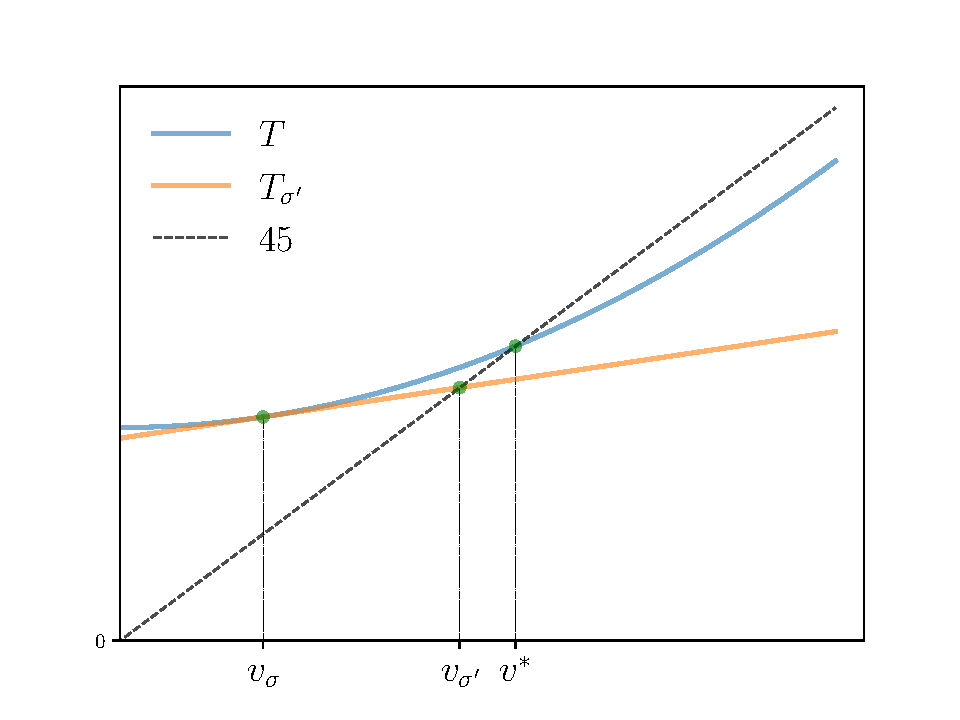
\includegraphics{howard_newton_1.pdf}}
        \caption{\label{f:howard_newton_1} HPI as a version of Newton's method}
    \end{figure}
    %

\end{frame}


\begin{frame}
    
    {\small
    \begin{algorithm}[H]
        \DontPrintSemicolon
        \vspace{0.2em}
        input $v_0$, an initial guess of $v^*$ \;
        \vspace{0.2em}
        input $\tau$, a tolerance level for error \;
        \vspace{0.2em}
        input $m \in \NN$, a step size \;
        \vspace{0.2em}
        $k \leftarrow 0$ \;
        \vspace{0.2em}
        $\epsilon \leftarrow +\infty$ \;
        \vspace{0.2em}
        \While{$\epsilon > \tau $}
        {
            \vspace{0.2em}
            $\sigma_k \leftarrow $ a $v_k$-greedy policy \;
            \vspace{0.2em}
            $v_{k+1} \leftarrow T_{\sigma_k}^m v_k$  \;
            \vspace{0.2em}
            $\epsilon \leftarrow \| v_k - v_{k+1} \|_\infty$ \;
            \vspace{0.2em}
            $k \leftarrow k + 1$ \;
            \vspace{0.2em}
        }
        \Return{$\sigma_k$}
        \vspace{0.2em}
        \caption{OPI}
    \end{algorithm}
    }

\end{frame}


\begin{frame}
    
    \vspace{0.4em}
    \vspace{0.4em}
    \vspace{0.4em}
    \begin{block}{\vspace*{-3ex}}
    {\bf Proposition.} Under the stated condition, VFI, HPI and OPI all converge
    \vspace{0.4em}
    \vspace{0.4em}

    Moreover, HPI converges to an exact optimal policy in finitely many steps
    \end{block}


    \vspace{0.4em}
    \vspace{0.4em}
    For details and proofs see Ch.\ 5 of \url{https://dp.quantecon.org/}


\end{frame}


\begin{frame}
    \frametitle{Modifications and extensions}

    Let's now look at some extensions to the basic model
    
\end{frame}





\begin{frame}
    
    We can switch to the \emp{expected value function}
    %
    \begin{equation*}
       g(x, a) 
             :=
             \sum_{x'} 
                v(x') P(x, a, x') 
    \end{equation*}

    with ``Bellman operator''
    %
    \begin{equation*}
        (Rg)(x, a)
        = 
         \sum_{x'} 
            \max_{a' \in \Gamma(x')}
            \left\{
                r(x', a')
                + \beta
                g(x', a')
            \right\}
            P(x, a, x') 
    \end{equation*}

        \vspace{0.5em}
        \vspace{0.5em}
        \vspace{0.5em}

    \begin{itemize}
        \item Does $R$ have the same properties as $T$?
        \vspace{0.5em}
        \item What are the equivalent algorithms and do they converge?
    \end{itemize}

\end{frame}

\begin{frame}
    
    We can introduce \emp{Epstein--Zin preferences}, as in
    %
    \begin{multline*}
        (Tv)(x) = \\
        \max_{a \in \Gamma(x)}
        \left\{
            r(x, a)^\alpha + \beta 
                \left(
                    \sum_{x'} v(x')^\gamma P(x,a, x')
                \right)^{\alpha / \gamma}
        \right\}^{1/\alpha}
    \end{multline*}


            \vspace{0.5em}
            \vspace{0.5em}
            \vspace{0.5em}
    \begin{itemize}
        \item Is $T$ still a contraction?
            \vspace{0.5em}
        \item Are the previous optimality results still valid?
            \vspace{0.5em}
        \item Do VFI, OPI, HPI converge?
    \end{itemize}

\end{frame}


\begin{frame}
    
    We can introduce \emp{risk-sensitive preferences}, as in
    %
    \begin{multline*}
        (Tv)(x) = \\
        \max_{a \in \Gamma(x)}
            \left\{
                r(x, a) + \beta \frac{1}{\theta} \ln 
                \left(
                    \sum_{x'} \exp(\theta v(x')) P(x, a, x')
                \right)
            \right\}
    \end{multline*}

            \vspace{0.5em}
            \vspace{0.5em}
            \vspace{0.5em}

    \begin{itemize}
        \item Is $T$ still a contraction?
            \vspace{0.5em}
        \item Are the previous optimality results still valid?
            \vspace{0.5em}
        \item Do VFI, OPI, HPI converge?
    \end{itemize}

\end{frame}


\begin{frame}
    
    We can introduce \emp{risk-sensitive preferences} with \emp{state-dependent
    discounting}, as in
    %
    \begin{multline*}
        (Tv)(x) = \\
        \max_{a \in \Gamma(x)}
            \left\{
                r(x, a) + \beta(x) \frac{1}{\theta} \ln 
                \left(
                    \sum_{x'} \exp(\theta v(x')) P(x, a, x')
                \right)
            \right\}
    \end{multline*}

            \vspace{0.5em}
            \vspace{0.5em}
            \vspace{0.5em}

    \begin{itemize}
        \item Is $T$ still a contraction?
            \vspace{0.5em}
        \item Are the previous optimality results still valid?
            \vspace{0.5em}
        \item Do VFI, OPI, HPI converge?
    \end{itemize}

\end{frame}


\begin{frame}
    
    Many, many extensions and combinations we can consider
    %
    \begin{itemize}
        \item ambiguity
            \vspace{0.5em}
        \item expected values in an Epstein--Zin framework
            \vspace{0.5em}
        \item expected values $+$ ambiguity $+$ state-dependent discounting
            \vspace{0.5em}
        \item integrated value functions in a risk-sensitive framework in
            continuous time
            \vspace{0.5em}
        \item $Q$-learning, etc., etc.
    \end{itemize}

            \vspace{0.5em}
            \vspace{0.5em}
            \vspace{0.5em}
    Is there any unifying theory?

            \vspace{0.5em}
    Or are all these problems too diverse?

\end{frame}




\begin{frame}
    \frametitle{Abstraction Level 1:  RDPs}

    \begin{enumerate}
        \item Construct a DP framework based on an
            abstraction of the Bellman equation
            \vspace{0.5em}
        \item State optimality results in this framework
            \vspace{0.5em}
        \item Connect with applications
    \end{enumerate}

    \vspace{0.5em}
    \vspace{0.5em}
    Builds on work by 
    %
    \begin{itemize}
        \item Eric Denardo 
        \vspace{0.5em}
        \item Dimitri Bertsekas 
        \vspace{0.5em}
        \item Takashi Kamihigashi
    \end{itemize}


\end{frame}



\begin{frame}
    \frametitle{Recursive Decision Problems}
    
    We begin with a generic version of the Bellman equation:
    %
    \begin{equation*}
        v(x) = \max_{a \in \Gamma(x)} B(x, a, v)
    \end{equation*}
    %

    %
    \begin{itemize}
        \item $x \in $ a finite set $\Xsf$ (the state space)
        \vspace{0.5em}
        \vspace{0.5em}
        \item $a \in $ a finite set $\Asf$ (the action space)
        \vspace{0.5em}
        \vspace{0.5em}
        \item $B(x, a, v) =$ total lifetime rewards
        \vspace{0.5em}
        \begin{itemize}
            \item contingent on current state-action pair $(x, a)$ 
            \vspace{0.5em}
            \item using  $v$ to evaluate future states
        \end{itemize}
    \end{itemize}


\end{frame}


\begin{frame}

    Formally, a \navy{recursive decision process} (RDP) is a triple
    %
    \begin{equation*}
     \rR = (\Gamma, V, B),
     \qquad \text{where...}
    \end{equation*}
   
            \vspace{0.5em}
            \vspace{0.5em}

    \navy{{\bf 1.}} $\Gamma$ is a nonempty correspondence from $\Xsf$ to $\Asf$
    %
    \begin{center}
        called the \navy{feasible correspondence}
    \end{center}

    which generates:
    %
    \begin{itemize}
        \item the \navy{feasible state-action pairs}
            %
            \begin{equation*}
                \Gsf := \setntn{(x, a) \in \Xsf \times \Asf}{a \in \Gamma(x)}
            \end{equation*}
            %
        \item the set of \navy{feasible policies}
            %
            \begin{equation*}
                \Sigma := 
                    \setntn{\sigma \in \Asf^\Xsf}
                    {\sigma(x) \in \Gamma(x) \text{ for all } x \in \Xsf}
            \end{equation*}
            %
    \end{itemize}

\end{frame}


\begin{frame}

    \navy{{\bf 2.}} $V$ is a subset of $\RR^\Xsf$ called the \navy{value space}

    \begin{itemize}
        \item[$\to$] candidates for the value function
    \end{itemize}


            \vspace{0.5em}
            \vspace{0.5em}
    
    \navy{{\bf 3.}} $B$ maps $\Gsf \times V$ to $\RR$,
     called the \navy{value aggregator}, satisfies

            \vspace{0.5em}
     (a) \navy{monotonicity}:
    %
    \begin{equation*}
        v \leq w \implies
        B(x, a, v) \leq B(x, a, w)
    \end{equation*}
    %

    (b) \navy{consistency}:
    %
    \begin{equation*}
        x \mapsto B(x, \sigma(x), v)
        \; \text{ is in $V$ whenever }
        \sigma \in \Sigma
        \text{ and }
        v \in V
    \end{equation*}
    %


\end{frame}




\begin{frame}
    
    \Eg Every MDP is an RDP 

    \vspace{0.5em}
    \vspace{0.5em}
    Take $\Gamma$ as given, set $V = \RR^\Xsf$, and 
    %
    \begin{equation*}
        B(x, a, v) = r(x, a) + \beta \sum_{x'} v(x') P(x, a, x')
    \end{equation*}
    %

    \vspace{0.5em}
    \begin{itemize}
        \item monotonicity and consistency conditions are trivial to check
        \vspace{0.5em}
        \item from $v(x) = \max_{a \in \Gamma(x)} B(x, a, v)$ we recover the MDP
        Bellman equation
        %
        \begin{equation*}
            v(x) = \max_{a \in \Gamma(x)} 
            \left\{
                r(x, a) + \beta \sum_{x'} v(x') P(x, a, x')
            \right\}
        \end{equation*}
        %
    \end{itemize}



\end{frame}


\begin{frame}
    

    \Eg Consider an \navy{optimal stopping} problem with 
    %
    \begin{equation*}
            v(x) = \max
            \left\{
                e(x), c(x) + \beta \sum_{x' \in \Xsf} v(x') P(x, x')
            \right\}
    \end{equation*}
    %

    \vspace{0.5em}
    \vspace{0.5em}
    Let $V = \RR^\Xsf$

    \vspace{0.5em}
    If $\Gamma(x) = \{0, 1\}$ and
    %
    \begin{equation*}
        B(x, a, v) = a e(x) + 
            (1-a) \left[
                c(x) + \beta \sum_{x' \in \Xsf} v(x') P(x, x')
            \right]
    \end{equation*}
    %
    
    then $(\Gamma, V, B)$ is an RDP with the same Bellman equation

\end{frame}


\begin{frame}
    
    \Eg Consider an MDP with \navy{state-dependent discounting}, so that
    %
    \begin{equation*}
            v(x)
            = \max_{a \in \Gamma(x)}
            \left\{
                r(x, a)
                + 
                \sum_{x'} v(x') \beta(x,a,x') P(x, a, x')
            \right\}
    \end{equation*}
    %

    \vspace{0.5em}
    \vspace{0.5em}
    Let $V = \RR^\Xsf$ and
    %
    \begin{equation*}
        B(x, a, v) 
        = r(x, a) + \sum_{x'} v(x') \beta(x, a, x') P(x, a, x')
    \end{equation*}
    %

    \vspace{0.5em}
    Now $(\Gamma, V, B)$ is an RDP with the same Bellman equation

\end{frame}


\begin{frame}
    
    \Eg Consider a modified MDP with \navy{risk-sensitive preferences}, so that
    %
    \begin{equation*}
        v(x) = \max_{a \in \Gamma(x)}
            \left\{
                r(x, a) + \beta \frac{1}{\theta} \ln 
                \left(
                    \sum_{x'} \exp(\theta v(x')) P(x, a, x')
                \right)
            \right\}
    \end{equation*}
    %
    for nonzero $\theta$

    \vspace{0.5em}
    \vspace{0.5em}
    With $V = \RR^\Xsf$ and 
    %
    \begin{equation*}
        B(x, a, v) =    
            r(x, a) + \beta \frac{1}{\theta} \ln 
            \left(
                \sum_{x'} \exp(\theta v(x')) P(x, a, x')
            \right)
    \end{equation*}
    %
    we obtain an RDP with the same Bellman equation

\end{frame}



\begin{frame}
    
    \Eg Consider a modified MDP with \navy{Epstein--Zin preferences}, so that
    %
    \begin{equation*}
        v(x) = \max_{a \in \Gamma(x)}
        \left\{
            r(x, a)^\alpha + \beta 
                \left(
                    \sum_{x'} v(x')^\gamma P(x,a, x')
                \right)^{\alpha / \gamma}
        \right\}^{1/\alpha}
    \end{equation*}
    %
    for nonzero $\alpha, \gamma$

    \vspace{0.5em}
    \vspace{0.5em}
    With $V = $ the strictly positive functions in $\RR^\Xsf$ and 
    %
    \begin{equation*}
        B(x, a, v) =    
        \left\{
            r(x, a)^\alpha + \beta 
                \left(
                    \sum_{x'} v(x')^\gamma P(x,a, x')
                \right)^{\alpha / \gamma}
        \right\}^{1/\alpha}
    \end{equation*}
    %
    we obtain an RDP with the same Bellman equation

\end{frame}


\begin{frame}
    
    \Eg Consider a modified MDP with \navy{quantile preferences}, so that
    %
    \begin{equation*}
        v(x) = \max_{a \in \Gamma(x)}
            \left\{
                r(x, a) + \beta (R^a_\tau v)(x)
            \right\}
    \end{equation*}
    %
     where
    %
    \begin{equation*}
        (R^a_\tau v)(x)
        := \text{$\tau$-th quantile of } 
        v(X') \text{ when } 
        X' \sim P(x, a, \cdot)
    \end{equation*}

    \vspace{0.5em}
    \vspace{0.5em}
    With $V = \RR^\Xsf$ and 
    %
    \begin{equation*}
        B(x, a, v) =    
                r(x, a) + \beta (R^a_\tau v)(x)
    \end{equation*}
    %
    we obtain an RDP with the same Bellman equation

\end{frame}




\begin{frame}
    
    \Eg Consider a \navy{shortest path problem} on graph $\gG = (\Xsf, E)$

    \vspace{0.5em}

    \begin{itemize}
        \item $c(x,x') =$ cost of traversing edge $(x,x') \in E$
        \vspace{0.5em}
        \item the direct successors of $x$ denoted by
            %
            \begin{equation*}
                \oO(x) := \setntn{x' \in \Xsf}{(x, x') \in E}   
            \end{equation*}
            %
    \end{itemize}
    

    \vspace{0.5em}
    \vspace{0.5em}
    \vspace{0.5em}
    Aim: find the minimum cost path from $x$ to a specified vertex $d$ 

    \vspace{0.5em}

    No discounting (so cannot use MDP theory)

\end{frame}



\begin{frame}

    The Bellman equation is
    %
    \begin{equation*}
        v(x) = \min_{x' \in \oO(x)} \{ c(x, x') + v(x') \}
    \end{equation*}
    %

    \vspace{0.5em}
    Let $V = \RR^\Xsf$

    \vspace{0.5em}
    \vspace{0.5em}
    Let $\Gamma(x) = \oO(x)$ and
    %
    \begin{equation*}
        B(x, x', v) = c(x, x') + v(x')  
    \end{equation*}
    %

    This is an RDP with the same Bellman equation

\end{frame}



\begin{frame}
    \frametitle{Policies}
    

    \vspace{0.5em}
    Consider an arbitrary RDP $(\Gamma, V, B)$
    \vspace{0.5em}

    A \navy{feasible policy} is a
    %
    \begin{equation*}
            \sigma \in \Asf^\Xsf
            \text{ such that }
            \sigma(x) \in \Gamma(x) \text{ for all } x \in \Xsf
    \end{equation*}
    %

    \vspace{0.5em}
    \vspace{0.5em}

    \begin{itemize}
        \item respond to state $X_t$ with action $\sigma(X_t)$ at 
        \emp{all} $t \geq 0$
        \vspace{0.5em}
        \vspace{0.5em}
        \item \navy{$\Sigma := $} the set of all feasible policies
    \end{itemize}



\end{frame}



\begin{frame}
    \frametitle{Policy Operators}

    Fix $\sigma \in \Sigma$ 

        \vspace{0.5em}
        \vspace{0.5em}
    The corresponding \navy{policy operator} $T_\sigma$ is
    defined at $v \in V$ by 
    %
    \begin{equation*}
        (T_\sigma \, v)(x)
        = B(x, \sigma(x), v)
        \qquad (x \in \Xsf)
    \end{equation*}
    %


        \vspace{0.5em}
        \vspace{0.5em}
        \vspace{0.5em}
        \vspace{0.5em}

        {\bf Lemma}.  $T_\sigma$ is an order-preserving self-map on $V$ 


        \vspace{0.5em}
        Proof: Immediate from monotonicity and consistency

\end{frame}


\begin{frame}
    

    \Eg The Epstein--Zin policy operator is 

    \begin{equation*}
    (T_\sigma \, v)(x) 
    =
        \left\{
            r(x, \sigma(x))^\alpha + \beta 
                \left(
                    \sum_{x'} v(x')^\gamma P(x,\sigma(x), x')
                \right)^{\alpha / \gamma}
        \right\}^{1/\alpha}
    \end{equation*}

\end{frame}

\begin{frame}
    \frametitle{Optimality}
    
    To define optimality for RDPs, we use the natural generalizations...

\end{frame}



\begin{frame}
    \frametitle{Lifetime value}


    Let $\rR := (\Gamma, V, B)$ be an RDP and let $\sigma$ be any policy
    
    \vspace{0.5em}
    \vspace{0.5em}
    Suppose $T_\sigma$ has a unique fixed point in $V$

    \vspace{0.5em}
    \vspace{0.5em}
    We denote this function by $v_\sigma$ and call it the \navy{$\sigma$-value
    function}

    \vspace{0.5em}
    \vspace{0.5em}
    We \underline{interpret} this function as the lifetime value of following
    $\sigma$

    \vspace{0.5em}
    \vspace{0.5em}
    \vspace{0.5em}

    We call $\rR$ \navy{well-posed} if $T_\sigma$ has a unique
    fixed point in $V$ for all $\sigma \in \Sigma$

\end{frame}


\begin{frame}

    \Eg Let $\rR$ be the RDP generated by an MDP

    \vspace{0.5em}
    \vspace{0.5em}
    Recall that 
    %
    \begin{equation*}
        T_\sigma \, v 
        = r_\sigma + \beta P_\sigma v
    \end{equation*}
    %


    \vspace{0.5em}
    This operator has the unique fixed point 
    %
    \begin{equation*}
        v_\sigma 
        = (I - \beta P_\sigma)^{-1} \, r_\sigma 
    \end{equation*}

    \vspace{0.5em}
    \vspace{0.5em}
    \vspace{0.5em}
    \begin{itemize}
        \item Hence $\rR$ is well-posed
        \vspace{0.5em}
        \item $v_\sigma(x) = \EE_x \sum_{t \geq 0} \beta^t r(X_t, \sigma(X_t))$
            $=$ lifetime value
    \end{itemize}

\end{frame}

\begin{frame}
    
    \Eg For the Epstein--Zin RDP, 
    %
    \begin{equation*}
        (T_\sigma v)(x) 
        =
        \left\{
            r(x, \sigma(x))^\alpha + \beta 
                \left[
                    \sum_{x' \in \Xsf} v(x')^\gamma P(x,\sigma(x), x')
                \right]^{\alpha / \gamma}
        \right\}^{1/\alpha}
    \end{equation*}
    %
    and 
    %
    \begin{center}
        $V := $ the strictly positive functions in $\RR^\Xsf$ 
    \end{center}


    \vspace{0.5em}
    \vspace{0.5em}

    \begin{itemize}
        \item Is this RDP well-posed?
    \end{itemize}

\end{frame}


\begin{frame}
    \frametitle{Greedy Policies}

    Fix $v \in \RR^\Xsf$ 
    
    \vspace{0.5em}
    \vspace{0.5em}
    A policy $\sigma$ is called \navy{$v$-greedy} if
    %
    \begin{equation*}
        \sigma(x)
        \in \argmax_{a \in \Gamma(x)}
            B(x, a, v)
    \end{equation*}
    %
    for all $x \in \Xsf$

    \vspace{0.5em}
    \vspace{0.5em}
    \vspace{0.5em}
    \vspace{0.5em}
    Note: at least one $v$-greedy policy exists in $\Sigma$


\end{frame}


\begin{frame}
    \frametitle{The Bellman Operator}
    

    \vspace{0.5em}
    The \navy{Bellman operator} is the self-map on $\RR^\Xsf$ defined by
    %
    \begin{equation*}
        (Tv)(x)
            = \max_{a \in \Gamma(x)}
            B(x, a, v)
    \end{equation*}
    %


    \vspace{0.5em}
    \vspace{0.5em}
    \vspace{0.5em}
    Key idea:

    \begin{equation*}
        Tv=v
        \quad \iff \quad
        v \text{ satisfies the Bellman equation}
    \end{equation*}

\end{frame}




\begin{frame}
    \frametitle{Optimality}

    Let $\rR$ be a well-posed RDP

    \vspace{0.5em}
    \vspace{0.5em}
    The \navy{value function} is defined by $v^* = \bigvee v_\sigma$


    \vspace{0.5em}
    \vspace{0.5em}
    More explicitly,
    %
    \begin{align*}
        v^*(x) 
        & := \max_{\sigma \in \Sigma} v_\sigma(x)
        \qquad (x \in \Xsf)
        \\
        & =  \text{max lifetime value from state $x$}
    \end{align*}
    %

    \vspace{0.5em}
    \vspace{0.5em}
    \vspace{0.5em}
    A policy $\sigma \in \Sigma$ is called \navy{optimal} if
    %
    \begin{equation*}
        v_\sigma = v^*
    \end{equation*}

\end{frame}


\begin{frame}[fragile]
    \frametitle{Howard policy iteration for RDPs}
    

    \begin{algorithm}[H]
        \DontPrintSemicolon
        input $\sigma_0 \in \Sigma$, an initial guess of $\sigma^*$ \;
        $k \leftarrow 0$ \;
        $\epsilon \leftarrow 1$ \;
        \While{$\epsilon > 0 $}
        {
            $v_k \leftarrow$ the unique fixed point of $T_{\sigma_k}$ \;
            $\sigma_{k+1} \leftarrow $ a $v_k$ greedy policy \;
            $\epsilon \leftarrow \1\{ \sigma_k \not= \sigma_{k+1} \}$ \;
            $k \leftarrow k + 1$ \;
        }
        \Return{$\sigma_k$}
    \end{algorithm}

\end{frame}


\begin{frame}
    
    Let $\rR$ be an RDP

    \vspace{0.5em}
    Key question:

    \vspace{0.5em}
    What assumptions to we need for optimality?

    \vspace{0.5em}
    Obviously $\rR$ must be well-posed

    \begin{itemize}
        \item each $T_\sigma$ has a unique fixed point in $V$
    \end{itemize}


    \vspace{0.5em}
    This is the \underline{minimum} requirement

    \vspace{0.5em}
    \vspace{0.5em}

    What else?

\end{frame}


\begin{frame}
    \frametitle{Stability}

    Let $\rR$ be an RDP
    
    \vspace{0.5em}
    \vspace{0.5em}
    \vspace{0.5em}
    We call $\rR$ \navy{globally stable} if, for all $\sigma \in \Sigma$,
    the operator $T_\sigma$ is globally stable on $V$

    \vspace{0.5em}
    \vspace{0.5em}
    \vspace{0.5em}
    \vspace{0.5em}

    That is, for all $\sigma \in \Sigma$,
    %
    \begin{enumerate}
        \item $T_\sigma$ has a unique fixed point $v_\sigma$ in $V$ and
        \vspace{0.5em}
        \vspace{0.5em}
        \item $\lim_{k \to \infty} T_\sigma^k v = v_\sigma$ for all $v \in V$
    \end{enumerate}


\end{frame}




\begin{frame}

    Let $\rR$ be a well-posed RDP with value function $v^*$

    \vspace{0.5em}
    \vspace{0.5em}
    \begin{block}{\vspace*{-3ex}}
        {\bf Theorem.} If $\rR$ is globally stable, then
        %
        \vspace{0.5em}
        \begin{enumerate}
            \item $v^*$ is the unique solution to the Bellman equation
                in $\RR^\Xsf$
            \vspace{0.5em}
            \item A feasible policy is optimal if and only it is
                $v^*$-greedy
            \vspace{0.5em}
            \item At least one optimal policy exists
            \vspace{0.5em}
            \item HPI returns an optimal policy in finitely
                many steps
            \vspace{0.5em}
            \item VFI and OPI converge
        \end{enumerate}
        %
    \end{block}

    \vspace{0.5em}

    Proof: See Ch~8

\end{frame}

\begin{frame}
    \frametitle{Types of RDPs}

    The optimality properties require global stability of all $T_\sigma$

        \vspace{0.5em}
    We can check this directly


        \vspace{0.5em}
    We can also 
    %
    \begin{enumerate}
        \item identify classes of RDPs that are globally stable
        \vspace{0.5em}
        \item show that a given application belongs to one of these classes
    \end{enumerate}


    
        \vspace{0.5em}
        \vspace{0.5em}
        \vspace{0.5em}

    Let's discuss the classification approach

        \vspace{0.5em}
        \vspace{0.5em}
    Below $\rR = (\Gamma, V, B)$ is a fixed RDP

\end{frame}

\begin{frame}
    \frametitle{Contracting RDPs}


        \vspace{0.5em}
    We call $\rR$ \navy{contracting} if $\exists \; \beta < 1$ such that
    %
    \begin{equation*}
       | B(x, a, v) - B(x, a, w)| 
       \leq \beta  \| v - w \|_\infty
    \end{equation*}
    %
   for all $(x, a) \in \Gsf \text{ and } v, w \in V$


        \vspace{0.5em}
        \vspace{0.5em}
   {\bf Thm}. If $\rR$ is contracting and $V$ is closed, then $\rR$ is
   globally stable


        \vspace{0.5em}
   Proof: Easy to show that each $T_\sigma$ is a contraction on $V$


        \vspace{0.5em}
        \vspace{0.5em}
        \vspace{0.5em}
   (Main idea dates back to Denardo 1967)


\end{frame}


\begin{frame}
    \frametitle{Eventually Contracting RDPs}
    

        \vspace{0.5em}
    We call $\rR$ \navy{eventually contracting} if 
    there is an $L \geq 0$ such that $\rho(L) < 1$ and 
    %
    \begin{equation*}
        |B(x, a, v)-B(x, a, w)|
        \leq \sum_{x'} |v(x') - w(x')| L(x, x')
    \end{equation*}
    %
   for all $(x, a) \in \Gsf \text{ and } v, w \in V$


        \vspace{0.5em}
        \vspace{0.5em}
        \vspace{0.5em}
   {\bf Thm}. If $\rR$ is eventually contracting and $V$ is closed, then $\rR$
   is globally stable


        \vspace{0.5em}
   Proof: See the book

\end{frame}



\begin{frame}
    \frametitle{Concave RDPs}
    
    We call $\rR$ \navy{concave} if
    %
    \begin{enumerate}
        \item  $V = [v_1, v_2]$ 
        \vspace{0.5em}
        \item $B(x, a, v_1) >  v_1(x) \text{ for all } (x, a) \in \Gsf$ and
        \vspace{0.5em}
        \item $v \mapsto B(x,a,v)$ is concave  for all $(x, a) \in \Gsf$
    \end{enumerate}


        \vspace{0.5em}
        \vspace{0.5em}
        \vspace{0.5em}
        \vspace{0.5em}
   {\bf Thm}. If $\rR$ is concave, then $\rR$
   is globally stable


        \vspace{0.5em}
   Proof: See the book

\end{frame}

\begin{frame}
    \frametitle{Application: job search with quantile preferences}

    Set up:
        \vspace{0.5em}
    \begin{itemize}
        \item wage offer process $(W_t)_{t \geq 0}$ is $P$-Markov on finite set $\Wsf$ 
        \vspace{0.5em}
        \item discount factor $\beta \in (0,1)$
    \end{itemize}

        \vspace{0.5em}
        \vspace{0.5em}
    The Bellman equation is
    %
    \begin{equation*}
        v(w) =
        \max
        \left\{
             \frac{w}{1-\beta} , \,   c + \beta (R_\tau v)(w) 
        \right\}
    \end{equation*}

    Here
    %
    \begin{equation*}
        (R_\tau v)(w)
        := \text{$\tau$-th quantile of } 
        v(W') \text{ when } 
        W' \sim P(w, \cdot)
    \end{equation*}

\end{frame}

\begin{frame}
    
    This problem studied in
        \vspace{0.5em}
    %
    \begin{itemize}
        \item de Castro and Galvao (2019)
        \vspace{0.5em}
        \vspace{0.5em}
        \item de Castro, Galvao and Nunes (2022)
        \vspace{0.5em}
        \vspace{0.5em}
        \item de Castro and Galvao (2022)
    \end{itemize}

\end{frame}

\begin{frame}
    
    We embed into the RDP framework by taking
    %
    \begin{itemize}
        \item $\Gamma(w) = \{0, 1\}$
        \vspace{0.5em}
        \item $V = \RR^\Wsf_+$
        \vspace{0.5em}
        \item $B$ given by 
            %
            \begin{equation*}
                B(w, a, v) 
                = a \frac{w}{1-\beta} + (1-a) [ c + \beta (R_\tau v)(w) ]
            \end{equation*}
            %
    \end{itemize}
    
        \vspace{0.5em}
        \vspace{0.5em}
        \vspace{0.5em}
    Easy to check that $\rR := (\Gamma, V, B)$ is an RDP with Bellman equation
    %
    \begin{equation*}
        v(w) =
        \max
        \left\{
             \frac{w}{1-\beta} , \,   c + \beta (R_\tau v)(w) 
        \right\}
    \end{equation*}


\end{frame}


\begin{frame}
    
    {\bf Proposition.}  $\rR$ is a contracting RDP

        \vspace{0.5em}
    \begin{itemize}
        \item Proof: See \href{https://dp.quantecon.org}{DP} Ch.~8
    \end{itemize}

        \vspace{0.5em}
        \vspace{0.5em}
        \vspace{0.5em}
    Since $V$ is closed, $\rR$ is globally stable 

        \vspace{0.5em}
    Hence all optimality properties apply

\end{frame}



\begin{frame}[fragile]
    
    \begin{figure}[H]
        \centering
        \scalebox{0.6}{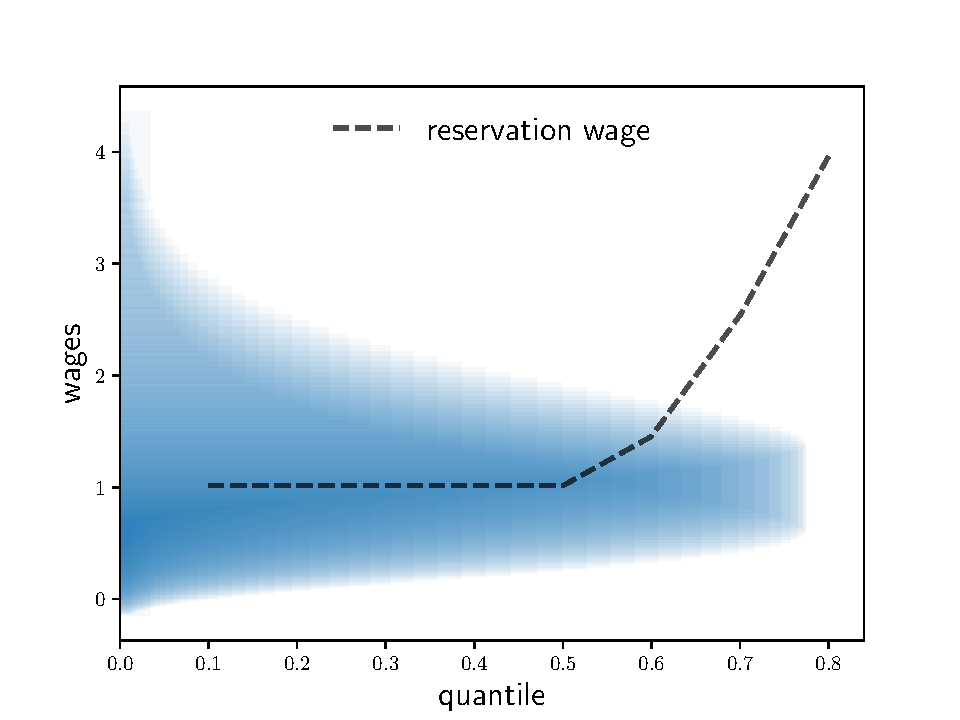
\includegraphics{quantile_js.pdf}}
    \end{figure}

\end{frame}





\begin{frame}
    \frametitle{Abstraction Level 2:  ADPs}
    
    We define an \navy{abstract dynamic program} (\navy{ADP}) to be a pair 
    %
    $$\aA = (V, \{T_\sigma\}_{\sigma \in \Sigma}), \qquad \text{where} $$
    %
    \vspace{-2.em}
    %
    \begin{enumerate}
        \item $V = (V, \preceq)$ is a partially ordered set and
            \vspace{0.5em}
        \item $\{T_\sigma\}_{\sigma \in \Sigma}$ is a family of self-maps on $V$
    \end{enumerate}
    %

            \vspace{0.5em}
            \vspace{0.5em}
            \vspace{0.5em}
    Below,

    \begin{itemize}
        \item elements of $\Sigma$ will be referred to as \navy{policies}
            \vspace{0.5em}
        \item elements of $\{T_\sigma \}$ are called \navy{policy operators}
    \end{itemize}

\end{frame}


\begin{frame}
    
    If $T_\sigma$ has a unique fixed point, then we
    %
    \begin{itemize}
        \item denote it $v_\sigma$ 
            \vspace{0.5em}
        \item call it the \navy{$\sigma$-value function}
    \end{itemize}

            \vspace{0.5em}
            \vspace{0.5em}
            \vspace{0.5em}

    Interpretation: 

    \begin{itemize}
        \item $V$ is a set of candidate value functions
            \vspace{0.5em}
        \item $\Sigma$ is a set of feasible policies
            \vspace{0.5em}
        \item the lifetime value of $\sigma \in \Sigma$ is $v_\sigma$
            \vspace{0.5em}
        \item we seek a greatest element in $\{v_\sigma\}_{\sigma \in \Sigma}$
    \end{itemize}


\end{frame}


\begin{frame}
    
    \Eg  Consider an RDP $(\Gamma, V, B)$
    %
            \vspace{0.5em}
            \vspace{0.5em}
            \vspace{0.5em}

    Let $\Sigma$ be the set of feasible policies

            \vspace{0.5em}
            \vspace{0.5em}
    Recall that, for each $\sigma \in \Sigma$ and $v \in V$,
    %
    \begin{equation*}
        (T_\sigma \, v)(x)
        = B(x, \sigma(x), v)
    \end{equation*}
    %

            \vspace{0.5em}
            \vspace{0.5em}
            \vspace{0.5em}

    The pair $(V, \{T_\sigma\})$ is an ADP

\end{frame}


\begin{frame}
    
    Recall the expected value Bellman equation
    %
    \begin{multline*}
        g(y, a)
        = \\
         \sum_{y'} \int
            \max_{a' \in \Gamma(y')}
            \left\{
                r(y', \epsilon', a')
                + \beta
                g(y', a')
            \right\}
            P(y, a, y') \phi(\epsilon') \diff \epsilon'
    \end{multline*}

    If $V = \RR^\Gsf$ and $R_\sigma$ is defined by 
    %
    \begin{multline*}
        (R_\sigma g)(y, a)
        = \\
         \sum_{y'} \int
            \left\{
                r(y', \epsilon', \sigma(y))
                + \beta
                g(y', \sigma(y))
            \right\}
            P(y, a, y') \phi(\epsilon') \diff \epsilon'
    \end{multline*}
    %
    then $(V, \{R_\sigma\})$ is an ADP

\end{frame}


\begin{frame}
    \frametitle{Benefits of ADP theory}
    

    \begin{itemize}
        \item More abstraction means easier proofs
            \vspace{0.5em}
            \vspace{0.5em}
            \vspace{0.5em}
        \item Removing structure makes it easier to see connections
            \vspace{0.5em}
            \vspace{0.5em}
            \vspace{0.5em}
        \item Can handle a more diverse range of problems
    \end{itemize}


\end{frame}

\begin{frame}
    
    Given $v \in V$, a policy $\sigma$ in $\Sigma$ is called \navy{$v$-greedy}
    if 
    %
    \begin{equation}\label{eq:adpg}
        T_{\sigma} \, v \succeq T_\tau \, v
        \quad \text{for all } \tau \in \Sigma
    \end{equation}

            \vspace{0.5em}
            \vspace{0.5em}
    \Eg For an RDP we have
    %
    \begin{equation*}
        (T_\sigma \, v)(x) 
            = B(x, \sigma(x), v)
    \end{equation*}
    %
    so \eqref{eq:adpg} holds iff 
    %
    \begin{equation*}
        \sigma(x) \in \argmax_{a \in \Gamma(x)} 
        B(x, a, v)
        \quad \text{for all } x \in \Xsf
    \end{equation*}


    \begin{itemize}
        \item ADP definitions generalize RDP definitions
    \end{itemize}

\end{frame}

\begin{frame}
    \frametitle{Bellman equation}
    
    Fix an ADP $\aA = (V, \{T_\sigma\})$

            \vspace{0.5em}
            \vspace{0.5em}
            \vspace{0.5em}
    We define the \navy{Bellman operator}  via
    %
    \begin{equation*}
        T v := \bigvee_\sigma T_\sigma \, v 
    \end{equation*}
    %
    (if it exists)


            \vspace{0.5em}
            \vspace{0.5em}
    We say that $v \in V$ satisfies the \navy{Bellman equation} if $T v=v$



\end{frame}



\begin{frame}
    \frametitle{Properties}
    
    We say that $\aA = (V, \{T_\sigma\})$ is
    
    \begin{itemize}
        \item \navy{well-posed} if $T_\sigma$ has one fixed point in
            $V$ for each $\sigma \in \Sigma$
            \vspace{0.5em}
            \vspace{0.5em}
        \item \navy{order stable} if $(V, T_\sigma)$ is order stable for each
            $\sigma \in \Sigma$
            \vspace{0.5em}
            \vspace{0.5em}
        \item \navy{max-stable} if $\aA$ is order stable, each $v \in V$ has at
            least one greedy policy, and $T$ has at least one fixed point in
            $V$
    \end{itemize}
    %

            \vspace{0.5em}
            \vspace{0.5em}
            \vspace{0.5em}
    Note: order stability is a regularity property --- see Ch~9

\end{frame}


\begin{frame}

    Let $\aA$ be a well-posed ADP 

            \vspace{0.5em}
            \vspace{0.5em}
    A policy $\sigma \in \Sigma$ is called \navy{optimal} for $\aA$ if
    %
    \begin{equation*}
        v_\tau \preceq v_\sigma
        \text{ for all }
        \tau \in \Sigma
    \end{equation*}

            \vspace{0.5em}
            \vspace{0.5em}
    We set $v^* := \bigvee_\sigma v_\sigma$ and call
    $v^*$ the \navy{value function}

            \vspace{0.5em}
            \vspace{0.5em}
    We define a self-map $H$ on $V$ via
    %
    $$ 
    H \, v = v_\sigma
    \quad \text{where} \quad 
    \text{$\sigma$ is $v$-greedy}
    $$

            \vspace{0.5em}
            \vspace{0.5em}
    Iterating with $H$ is an abstract version of HPI

\end{frame}


\begin{frame}
    \frametitle{Max-Optimality}
    
    \begin{block}{\vspace*{-3ex}}
        {\bf Theorem.} If $\aA$ is max-stable, then 
        %
                \vspace{0.5em}
        \begin{enumerate}
            \item $v^*$ exists in $V$ 
                \vspace{0.5em}
            \item $v^*$ is the unique solution to the Bellman equation in $V$ 
                \vspace{0.5em}
            \item a policy is optimal if and only if it is $v^*$-greedy
                \vspace{0.5em}
            \item at least one optimal policy exists
        \end{enumerate}
        %
                \vspace{0.5em}
                \vspace{0.5em}
        If, in addition, $\Sigma$ is finite, then HPI $\to v^*$ in finitely many steps
    \end{block}



    Proof: See Ch.~9

\end{frame}



\begin{frame}
    \frametitle{Subordinate ADPs}


    Let $\aA := (V, \{T_\sigma\})$ and $\hat \aA := (\hat V, \{\hat T_\sigma\})$ be
    ADPs

            \vspace{0.5em}
            \vspace{0.5em}
            \vspace{0.5em}
    We say that $\hat \aA$ is \navy{subordinate} to $\aA$ if $\exists$ 
    %
    \begin{enumerate}
        \item an order-preserving map $F$ from $V$ onto $\hat V$ and
            \vspace{0.5em}
        \item order-preserving maps $\{G_\sigma\}_{\sigma \in \Sigma}$ from
            $\hat V$ to $V$
    \end{enumerate}

            \vspace{0.5em}
    such that
    %
    \begin{equation*}
        T_\sigma = G_\sigma \circ F
        \quad \text{and} \quad
        \hat T_\sigma = F \circ G_\sigma 
        \qquad \text{ for all } \sigma \in \Sigma
    \end{equation*}
    %


    Let $G = \bigvee_\sigma G_\sigma$

\end{frame}


\begin{frame}
    
    {\bf Theorem.}
    If 
    %
    \begin{enumerate}
        \item $\aA$ is max-stable and
        \item $\hat \aA$ is subordinate to $\aA$, 
    \end{enumerate}
    %
    then 
    $\hat \aA$ is also max-stable and the Bellman operators are related by
    %
    \begin{equation*}
        T = G \circ F
        \quad \text{and} \quad
        \hat T = F \circ G
    \end{equation*}
    %
    while  the value functions are related by 
    %
    \begin{equation*}
        v^* = G \, \hat v^*
        \quad \text{and} \quad
        \hat v^* = F \, v^*
    \end{equation*}
    %
    Moreover, 
    %
    \begin{enumerate}
        \item if $\sigma$ is optimal for $\aA$, then $\sigma$ is optimal
            for $\hat \aA$, and
        \item if $G_\sigma \, \hat v^* = G \, \hat v^*$, then $\sigma$ is
            optimal for $\aA$
    \end{enumerate}
    %

\end{frame}


\begin{frame}
    \frametitle{Application}
    
    Consider an Epstein--Zin dynamic program with Bellman equation
    %
    \begin{equation*}
        v(w, e) = 
        \max_{0 \leq s \leq w}
            \left\{
                r(w, s, e)^\alpha + \beta 
                \left( \sum_{e'} v(s, e')^\gamma \phi(e') \right)^{\alpha/ \gamma}
            \right\}^{1/\alpha}
    \end{equation*}
    %

    Here 
    %
    \begin{itemize}
        \item $w$ is current wealth (discretized)
            \vspace{0.5em}
        \item $s$ is savings (discretized)
            \vspace{0.5em}
        \item $e$ is an {\sc iid} endowment shock with range $\Esf$  
            \vspace{0.5em}
        \item $\beta$ is a constant in $(0,1)$ and $r$ is a reward function
    \end{itemize}


\end{frame}

\begin{frame}
    
    The policy operator corresponding to $\sigma \in \Sigma$ is
    %
    \begin{equation*}
        (T_\sigma \, v)(w, e) = 
            \left\{
                r(w, \sigma(w), e)^\alpha + \beta 
                \left( \sum_{e'} v(\sigma(w), e')^\gamma \phi(e') \right)^{\alpha/ \gamma}
            \right\}^{1/\alpha}
    \end{equation*}
    %

            \vspace{0.5em}
            \vspace{0.5em}
    {\bf Proposition.} If 
    %
    \begin{itemize}
        \item $\Xsf := \Wsf \times \Esf$ and 
        \item $V := (0, \infty)^\Xsf$, 
    \end{itemize}
    %
    then $\aA = (V, \{T_\sigma\})$ is a max-stable ADP


    (Details in Ch~9)

\end{frame}


\begin{frame}
    
Next consider the operator
%
\begin{equation*}
    (B_\sigma \, h)(w) = 
        \left\{
            \sum_e
            \left\{ 
                r(w, \sigma(w), e)^\alpha + \beta h(\sigma(w))^\alpha
            \right\}^{\gamma/\alpha}
             \phi(e)
        \right\}^{1/\gamma},
\end{equation*}
%
where $h$ is an element of $(0, \infty)^\Wsf$

            \vspace{0.5em}
            \vspace{0.5em}
Define $F$ at $v \in V$ by
%
\begin{equation*}
    (Fv)(w) = \left\{ \sum_{e} v(w, e)^\gamma \phi(e) \right\}^{1/\gamma}
        \qquad (w \in \Wsf)
\end{equation*}
%
            \vspace{0.5em}
            \vspace{0.5em}

Then $\bB = (F(V), \{B_\sigma\})$ is also an ADP

\end{frame}


\begin{frame}
    

    Moreover, $\bB$ is subordinate to $\aA$

            \vspace{0.5em}
            \vspace{0.5em}
            \vspace{0.5em}
    To see, this, define $G_\sigma$  by
    %
    \begin{equation*}
        (G_\sigma \, h)(w, e) 
        = 
            \left\{
                r(w, \sigma(w), e)^\alpha + \beta 
                h(\sigma(w))^\alpha
            \right\}^{1/\alpha} 
    \end{equation*}
    %

    Then 
    %
    \begin{itemize}
        \item $F$ and $G_\sigma$ are order-preserving
            \vspace{0.5em}
        \item $T_\sigma$ is equal to $G_\sigma \circ F$ and 
            \vspace{0.5em}
        \item $B_\sigma$  is equal to $F \circ G_\sigma$ 
    \end{itemize}

\end{frame}


\begin{frame}
    

    \begin{algorithm}[H]
    \DontPrintSemicolon
    input $\sigma_0 \in \Sigma$, set $k \leftarrow 0$ and $\epsilon \leftarrow 1$ \;
    \While{$\epsilon > 0 $}
    {
        $h_k \leftarrow $ the fixed point of $B_{\sigma_k}$ \;
        $\sigma_{k+1} \leftarrow $ an $h_k$-greedy policy, satisfying
        %
        \begin{equation*}
            \sigma_{k+1}(w) \in \argmax_{0 \leq s \leq w}
            \left\{
                \sum_e
                \left\{ 
                    r(w, s, e)^\alpha + \beta h(s)^\alpha
                \right\}^{\gamma/\alpha}
                 \phi(e)
            \right\}^{1/\gamma}
        \end{equation*}
        %
        \;
        \vspace{-1em}
        $\epsilon \leftarrow \1\{ \sigma_k \not= \sigma_{k+1} \}$ and $k \leftarrow k + 1$ \;
    }
    Compute $\sigma$ to satisfy
    %
    $$
        \sigma(w, e) \in
        \argmax_{0 \leq s \leq w}
        \left\{
            r(w, s, e)^\alpha + \beta 
            h_k(s)^{\alpha}
        \right\}^{1/\alpha} 
    $$ \;
    \vspace{-2em}
    \Return{$\sigma$}
    \caption{Solving $\aA$ via $\bB$}
\end{algorithm}

\end{frame}


\begin{frame}
    
\begin{figure}
   \centering
   % trim l b r t
   \scalebox{0.4}{ 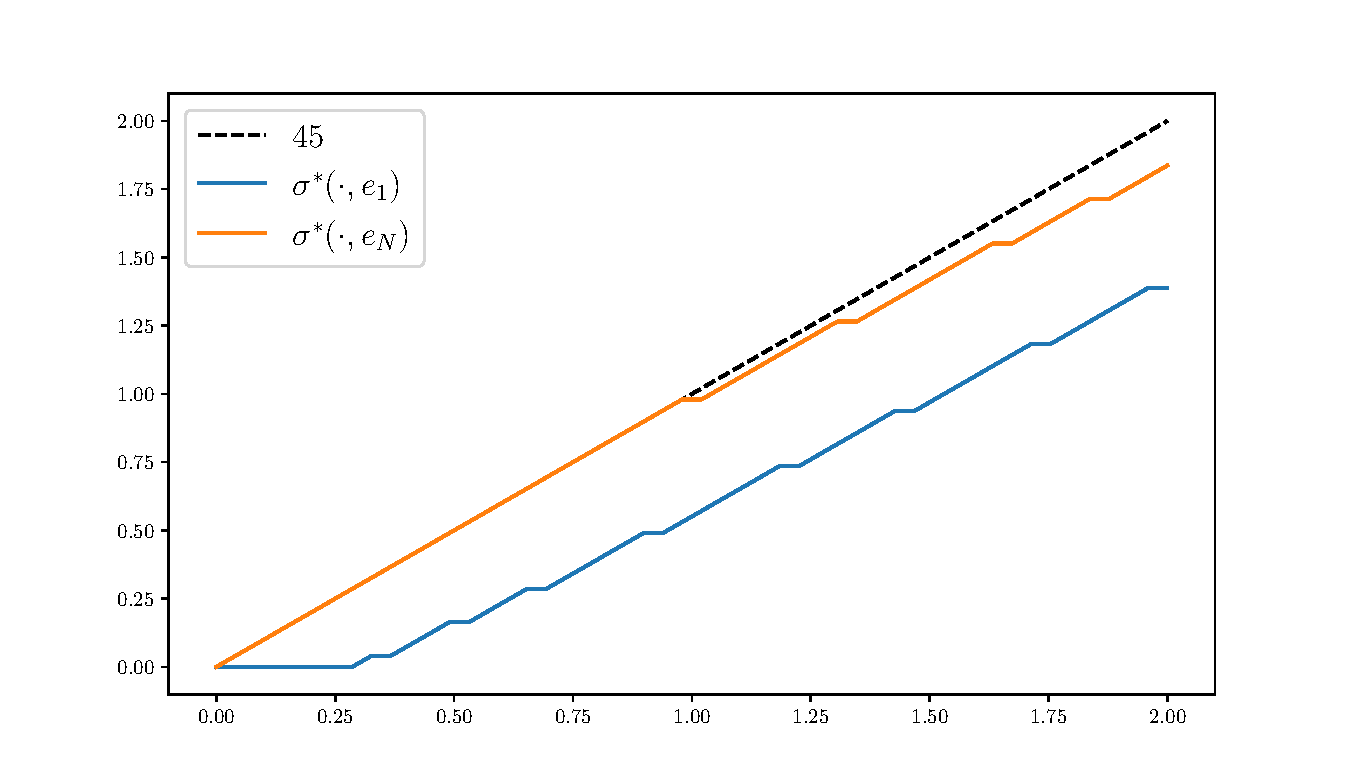
\includegraphics[trim = 0mm 0mm 0mm 0mm, clip]{policies.pdf}}
   \caption{\label{f:policies} Optimal savings policy with Epstein--Zin
   preference}
\end{figure}


\end{frame}

\begin{frame}
    
\begin{figure}
   \centering
   % trim l b r t
   \scalebox{0.4}{ 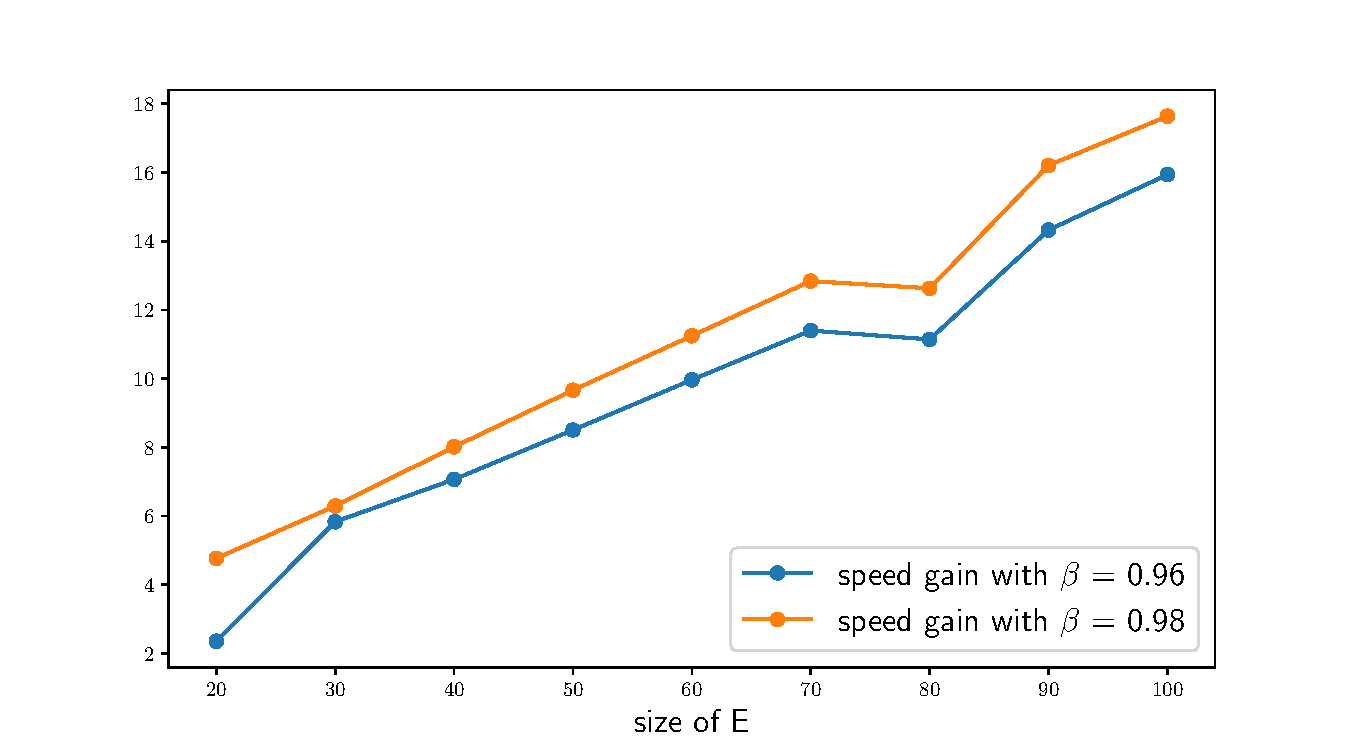
\includegraphics[trim = 0mm 0mm 0mm 0mm, clip]{rel_timing.pdf}}
   \caption{\label{f:rel_timing} Speed gain from replacing $\aA$ with
   subordinate model $\bB$ }
\end{figure}

\end{frame}


\begin{frame}
    
    For details of computations see

    \begin{center}
        \url{https://github.com/jstac/adps_public}
    \end{center}

\end{frame}


\end{document}









